\chapter{Results}
\label{ch:results}

Describe your results here...

Results are typically accompanied by tables and figures. These are, in \LaTeX, so-called ``floating environments'', meaning they are placed where they look nice, typically on the next page, top, or, if there is enough space, this page, bottom.


\begin{table}
	\caption{The caption of a table always goes \emph{above} the table.} \label{tab:example}	
	\centering
	\begin{tabular}{lcr} % alignment: left, centre, right
		\hline
		effect  & df  & $P$-value \\ \hline
		rain    & 1   & $<0.001$ \\
		human population density & 1 & $0.051$ \\
		residuals & 5223 &  \\ \hline
	\end{tabular}
\end{table}

The table is a bit of a nightmare in \LaTeX, unless you use the editor's help to construct a template. Here (Table~\ref{tab:example}) is a simple table in a floating environment. Note how nicely you can refer to figures using labels and referencing.
For tricks on how to merge columns or landscape tables or multi-page tables or define the widths of a column or use different line types for top and bottom, please search the internet: it is all possible, somehow.

And here an example of a floating picture (Fig.~\ref{fig:example}). The more text you write, the better the floating objects are separated. So don't let this ugly example deter you. 

You can try to force \LaTeX\/ to place a float HERE, but typically this does not improve the output and is against the ``philosophy'' of not investing time into the layout itself.

\begin{figure}
	\centering
	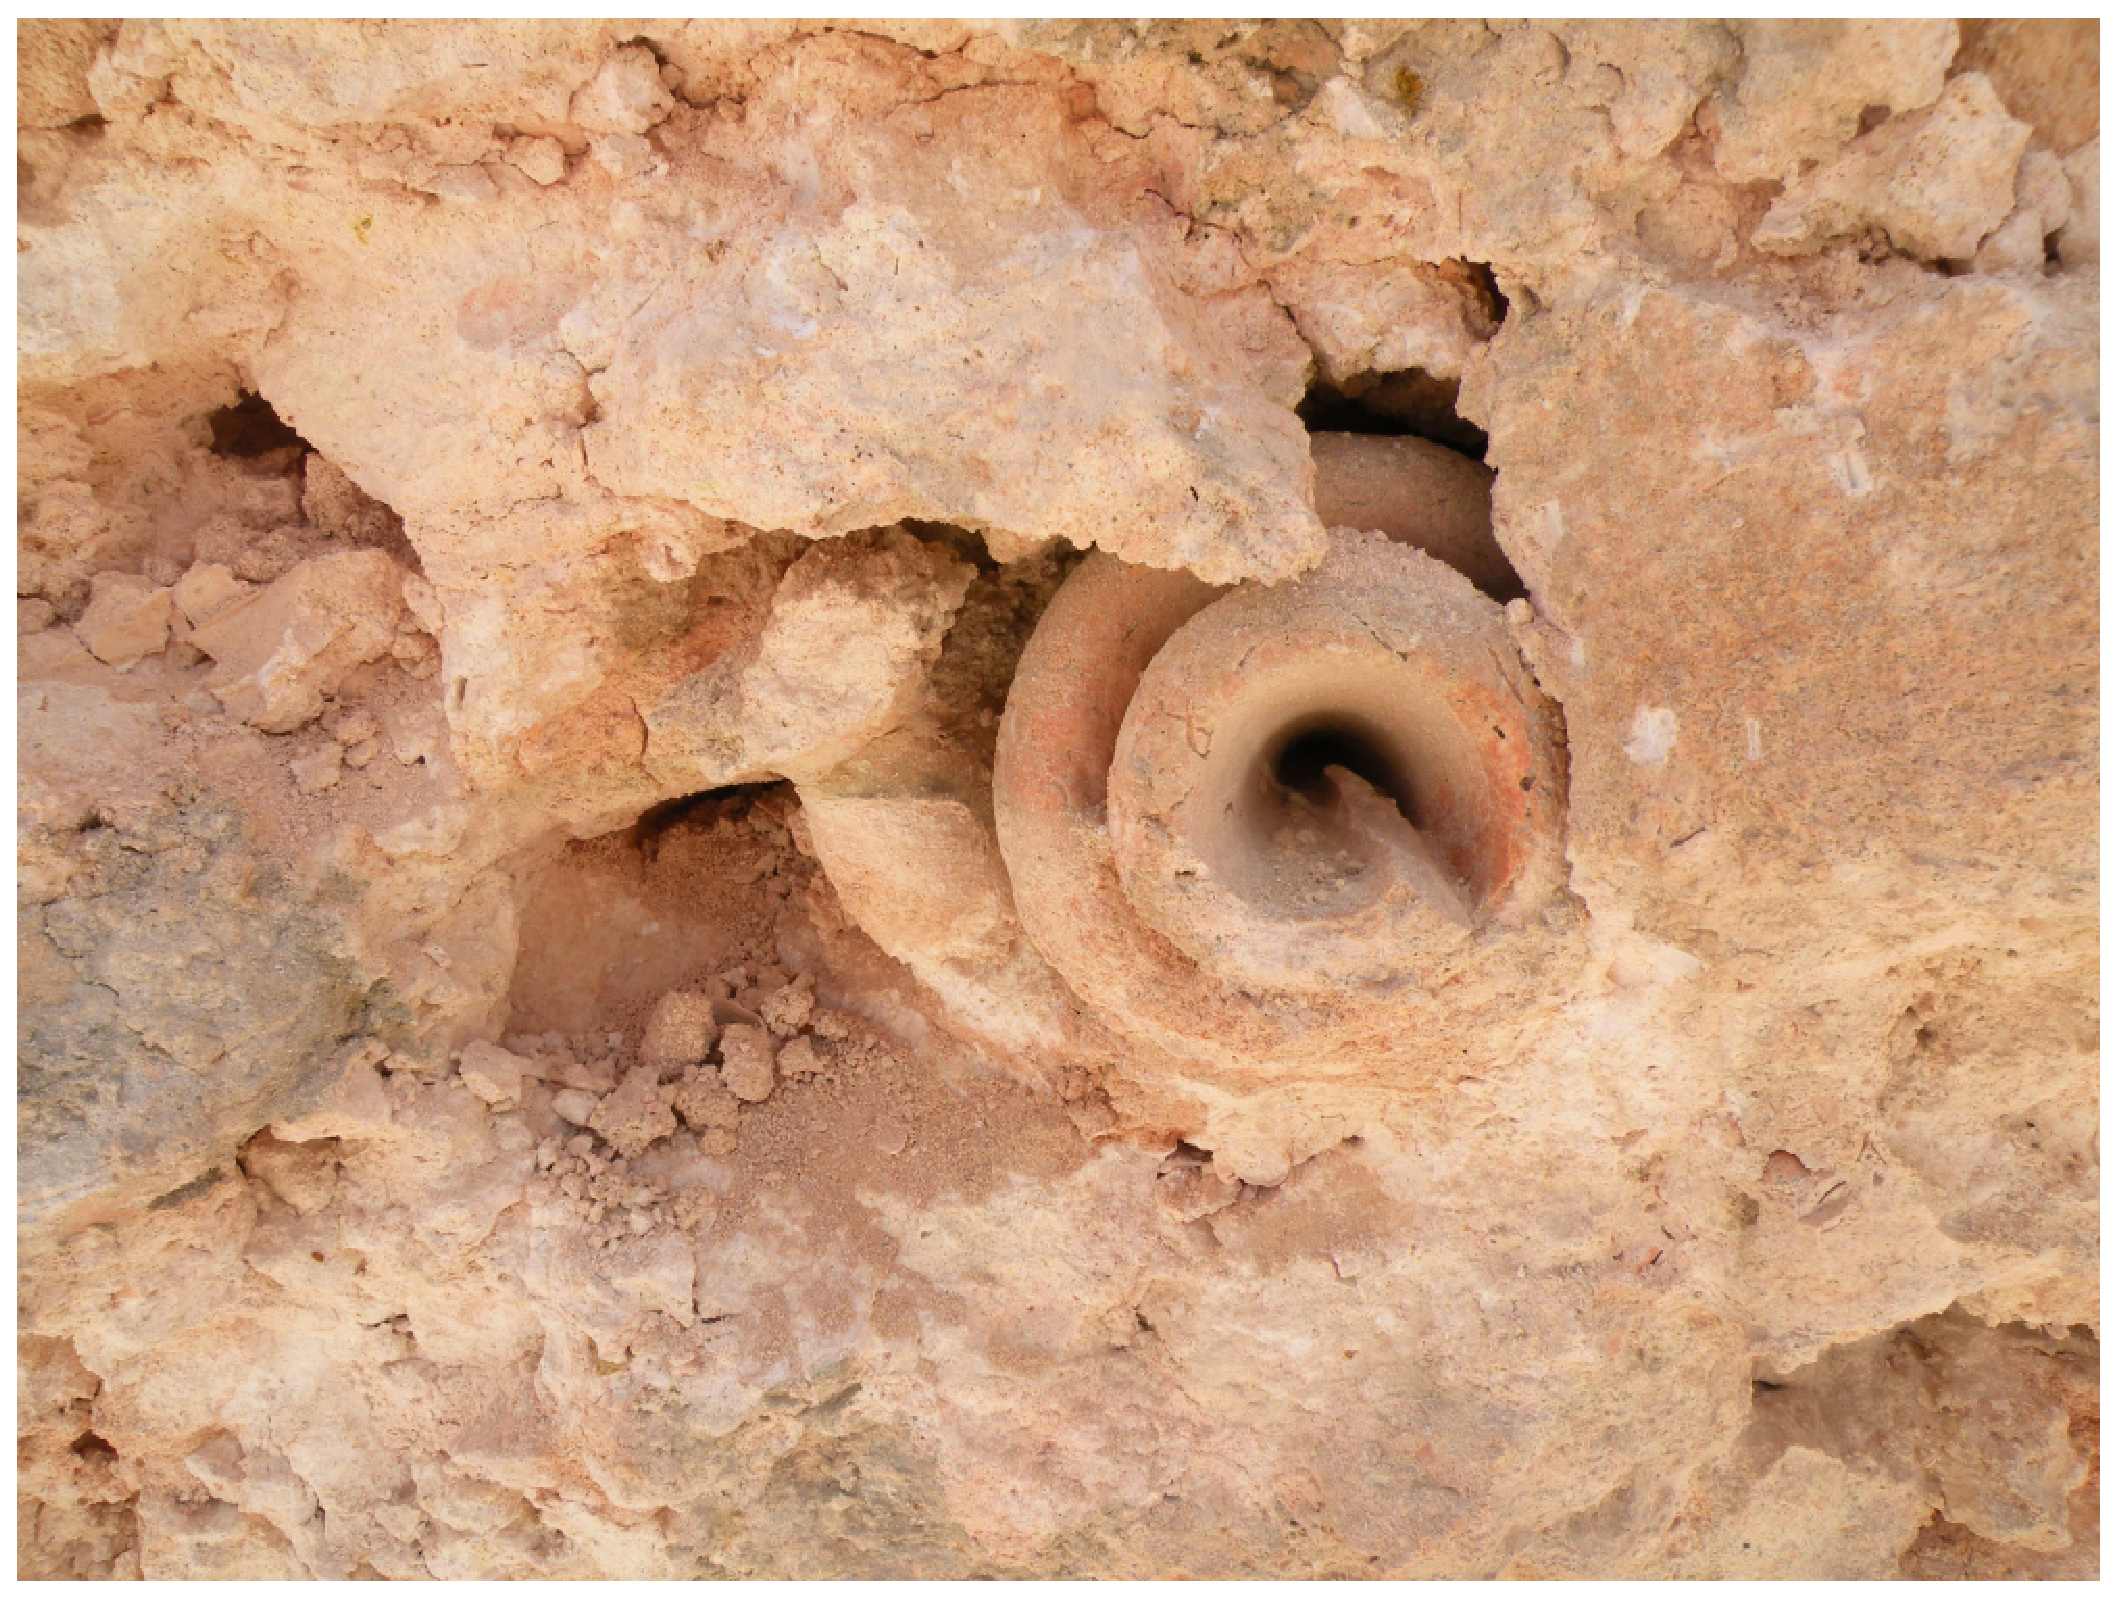
\includegraphics[width=0.5\textwidth]{images/bsc-fossil}
	\caption{The caption of a figure always goes \emph{below} the figure: we wouldn't pay attention to text, if there is a picture to look at!} \label{fig:example}
\end{figure}